\documentclass{beamer}

\usepackage{tikz}
\usepackage[labelfont=bf]{caption}
\usepackage{booktabs}
\usepackage{caption}
\usepackage{siunitx}
\usepackage{amsmath}
\usepackage{pgfplots}
\usepackage{pgfplotstable}

\title{Proving Conservation of Energy through relating Spring Potential and Kinetic Energy}
\author{Henry Oehlrich\and Chelsea Liao\and Shreyas Raychaudhuri}

\begin{document}
\maketitle

\begin{frame}
    \frametitle{Abstract}
    The objective of this experiment is to prove the concept of conservation of
    energy. This was done by relating spring potential energy to kinetic
    energy. After multiple trials of various initial potential energies, it was
    concluded that the concept of conservation of energy holds true.
\end{frame}

\begin{frame}
    \frametitle{Experiment Setup}
    \begin{figure}
        \centering
        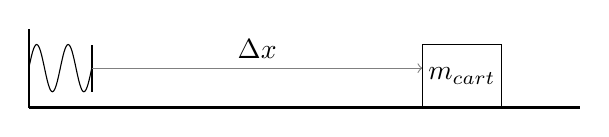
\begin{tikzpicture}
            \draw[thick] (0,0) -- (7,0);
            \draw[thick] (0,0) -- (0,1);
            \draw (0,0.5) sin (0.1,0.8) cos (0.2,0.5) sin (0.3,0.2) cos (0.4,0.5) sin (0.5,0.8)
                cos (0.6,0.5) sin (0.7,0.2) cos (0.8,0.5);
            \draw[thick] (0.8,0.2) -- (0.8,0.8);
            \draw[->,gray] (0.8,0.5) -- (5,0.5);
            \draw[rectangle,color=black] (5,0) rectangle (6,0.8) node[midway] {$m_{cart}$};
            \draw (2.9,0.5) node[above] {$\Delta x$};
        \end{tikzpicture}
    \end{figure}
    \begin{figure}
        \centering
        \begin{tabular}{l|l|l}
            \toprule
            Symbol & Description &  Value \\
            \midrule
            $m_{cart}$ & cart mass & \qty{0.285}{\kg} \\
            $k$ & spring constant & 8 \\
            $\Delta x$ & extension dist & varies \\
            $v$ & final velocity & measured \\
        \end{tabular}
    \end{figure}
\end{frame}

\begin{frame}
    \frametitle{Materials and Methods}
    The experiment setup consisted of a cart on a track with a spring attached
    to the end of the track. The cart was pulled back a certain distance and
    released. This was repeated for different distances. The final velocity of
    the cart was measured using an accelerometer on the cart. We conducted 11
    trials with distances ranging from \qty{0.1}{\m} to \qty{0.5}{\m} in
    increments of \qty{0.1}{\m}.
\end{frame}

\begin{frame} 
    \frametitle{Results} 
    A regression analysis was done between calculated spring potential energy
    and measured kinetic energy. The $R^2$ of 99.5\% shows that only 0.5\% of
    the variance in final kinetic energy is not explained by initial spring
    energy. From this, we can conclude that this experiment supports the
    concept of conservation of energy.
\end{frame}

\begin{frame}
    \frametitle{Energy Relationship Graph}
    \begin{tikzpicture}
        \begin{axis}[
                xlabel={Spring Potential Energy (\si{\joule})},
                ylabel={Final Kinetic Energy (\si{\joule})},
                width=0.8\textwidth,
            ]
            \addplot +[only marks,mark size=1.5pt] table
            {xy.dat};
            \addplot table [
                y={create col/linear regression={y=k}},
                mark=none,
            ]
            {xy.dat};
        \end{axis}
    \end{tikzpicture}
\end{frame}

\begin{frame}
    \frametitle{Discussion}
    \begin{itemize}
        \item Although the data were very strongly correlated, for each trial,
            the final kinetic energy was slightly less than the initial spring
            potential energy. This could be due to friction in the system.
        \item The loss in kinetic energy could also be attributed to
            degradation of the spring after measuring the spring constant.
        \item This experiment could be improved by eliminating work done by
            friction in the system and by using a more consistent spring.
    \end{itemize}
\end{frame}

\end{document}
